\documentclass[11pt]{article}

\usepackage[utf8]{inputenc}
\usepackage[T1]{fontenc}
\usepackage{indentfirst}
\usepackage{titlesec}
\usepackage{float}
\usepackage{multirow}

\usepackage{listings}
\usepackage{color}

\lstset{
language=bash,                % choose the language of the code
basicstyle=\footnotesize,       % the size of the fonts that are used for the code
numbers=left,                   % where to put the line-numbers
numberstyle=\footnotesize,      % the size of the fonts that are used for the line-numbers
stepnumber=1,                   % the step between two line-numbers. If it is 1 each line will be numbered
numbersep=5pt,                  % how far the line-numbers are from the code
backgroundcolor=\color{white},  % choose the background color. You must add \usepackage{color}
showspaces=false,               % show spaces adding particular underscores
showstringspaces=false,         % underline spaces within strings
showtabs=false,                 % show tabs within strings adding particular underscores
frame=single,           % adds a frame around the code
tabsize=2,          % sets default tabsize to 2 spaces
captionpos=b,           % sets the caption-position to bottom
breaklines=true,        % sets automatic line breaking
breakatwhitespace=false,    % sets if automatic breaks should only happen at whitespace
escapeinside={\%*}{*)}          % if you want to add a comment within your code
}

\titlelabel{\thetitle.\quad}

\renewcommand{\lstlistingname}{Programski odsječak}
\renewcommand{\figurename}{Slika}
\renewcommand{\tablename}{Tablica}

%Gummi|063|=)
\title{\textbf{2. domaća zadaća}\\
		Paralelno programiranje}
\author{Matija Šantl \\
		0036458898}	
\date{}
\usepackage{graphicx}
\begin{document}

\maketitle

\section{Zadatak}
Uporabom MPI-a ostvariti program za igranje igre \lq\lq{}4 u nizu\rq\rq{} uz gravitaciju za jednog igrača (čovjek protiv računala). Kao rezultat domaće zadaće potrebno je tablično i grafički prikazati ubrzanje i učinkovitost algoritma za $p$ procesora pri čemu je $p = 1, 2, 3, 4, 5, 6, 7, 8$.

\section{Paralelni algoritam}

Ostvarenje paralelnog algoritma napravljena je po uzoru na model voditelj-radnik.

U nastavku su opisane četiri faze razvoja.

\subsection{Podjela}
Podjela podataka je vršena na sljedeći način. Svaki radnik kao ulaz dobije trenutno stanje ploče, oznaku stupca nad kojim je izvršen potez, oznaku igrača koji je obavio taj potez te dubina do koje se pretražuje stablo odluke. \label{voditelj}

Podjela izračunavanja je vrlo jednostavna. Voditelj dodijeli svakom radniku stanje ploče, potez i dubinu do koje on onda vrši izračun, tj. svaki radnik izračunava ishod igre za jedan od mogućih poteza.

\subsection{Komunikacija}
Komunikacija je ostvarena po uzoru na voditelj-radnik model. Voditelj šalje potrebne podatke radnicima (kako je opisano u \ref{voditelj}), dok svaki radnik vraća voditelju odgovor u obliku jedne poruke koja sadrži potrebne identifikatore igrača i stupca te skalarnu vrijednost koja je proporcionalna isplativosti igranja poteza tog igrača nad tim stupcem.

\subsection{Aglomeracija}
Broj zadataka ovisi o dimenzijama ploče i dubini pretraživanja stabla odluke. Ukupni broj zadataka koji se stvara za odlučivanje najboljeg poteza računala za određenu dubinu je $\log_{2} (dubina) \cdot stupaca$.

\subsection{Pridruživanje}
Računalo na kojem je paralelni algoritam izvođen ima sljedeće karakteristike.

\begin{lstlisting}[caption=cat /proc/cpuinfo]
processor       : 0
vendor_id       : GenuineIntel
model name      : Intel(R) Xeon(R) CPU           E5645  @ 2.40GHz
cpu MHz         : 2394.192
...
processor       : 23
vendor_id       : GenuineIntel
model name      : Intel(R) Xeon(R) CPU           E5645  @ 2.40GHz
cpu MHz         : 2394.192
\end{lstlisting}

Budući da su sustav i zadaci homogeni, kod pridruživanja se nije obraćala pažnja koji procesor će izvršavati koji zadatak.

\section{Upute}
Izvorni tekst paralelnog algoritma je organiziran po sljedećim elementima:
\begin{itemize}
\item board.c, board.h\\ Funkcije i strukture podataka koje nam olakšavaju operacije nad igračom pločom.
\item list.c, list.h\\ Struktura podataka jednostruko povezana lista koju voditelj koristi kako bi znao koji radnici su slobodni.
\item main.c\\ Ostvarenje paralelnog algoritma.
\item Makefile\\ Pravila kojima se automatizira prevođenje i povezivanje izvornog teksta.
\item run.sh\\ Skripta koja pokreće paralelni algoritam s različitim parametrima (broj procesora, dubina pretraživanja) te sprema vremena izvođenja u za to predviđene datoteke.
\end{itemize}

U nastavku su dane upute o pokretanju programa ovisno o ulaznim parametrima.

\begin{lstlisting}[caption=Prevođenje i pokretanje paralelnog algoritma]
$ make
$ mpirun -n BROJ_PROCESORA ./connect4 DUBINA_PRETRAZIVANJA
\end{lstlisting}

\section{Učinkovitost algoritma}
U nastavku je dan prikaz vremena izvođenja paralelnog algoritma tablično i grafom.

\begin{table}[h]
\begin{tabular}{cc|c|c|c|c|c|c|c|l}
\cline{3-9}
& & \multicolumn{7}{ c| }{Dubina pretraživanja} \\ \cline{3-9}
& & 4 & 5 & 6 & 7 & 8 & 9 & 10 \\ \cline{1-9}
\multicolumn{1}{ |c| }{\multirow{8}{*}{Broj procesora} } &
\multicolumn{1}{ |c| }{1} & 0.0035 & 0.02200 & 0.1443 & 0.9427 & 6.1669 & 39.7422 & 254.9565 &     \\ \cline{2-9}

\multicolumn{1}{ |c  }{}                        &
\multicolumn{1}{ |c| }{2} & 0.0021 & 0.0126 & 0.0818 & 0.5307 & 3.4615 & 22.1848 & 142.3800 &     \\ \cline{2-9}

\multicolumn{1}{ |c  }{}                        &
\multicolumn{1}{ |c| }{3} & 0.0018 & 0.0095 & 0.0627 & 0.4185 & 2.6376 & 16.6265 & 105.7949 &     \\ \cline{2-9}

\multicolumn{1}{ |c  }{}                        &
\multicolumn{1}{ |c| }{4} & 0.0041 & 0.0095 & 0.0496 & 0.2900 & 1.8708 & 11.7097 & 78.3599 &     \\ \cline{2-9}

\multicolumn{1}{ |c  }{}                        &
\multicolumn{1}{ |c| }{5} & 0.0011 & 0.0068 & 0.0424 & 0.2784 & 1.7527 & 11.7283 & 75.9025 &     \\ \cline{2-9}

\multicolumn{1}{ |c  }{}                        &
\multicolumn{1}{ |c| }{6} & 0.0017 & 0.0064 & 0.0433 & 0.2743 & 1.8233 & 11.0918 & 70.0235 &     \\ \cline{2-9}

\multicolumn{1}{ |c  }{}                        &
\multicolumn{1}{ |c| }{7} & 0.0022 & 0.0085 & 0.0301 & 0.1686 & 1.1677 & 9.6578 & 42.3355 &     \\ \cline{2-9}

\multicolumn{1}{ |c  }{}                        &
\multicolumn{1}{ |c| }{8} & 0.0029 & 0.0121 & 0.0344 & 0.2164 & 1.1267 & 8.8622 & 44.0685 &     \\ \cline{1-9}
\end{tabular}
\caption{Vremena izvođenja izražena u sekundama}
\end{table}

\clearpage

\begin{figure}[!htb]	
	\centering
	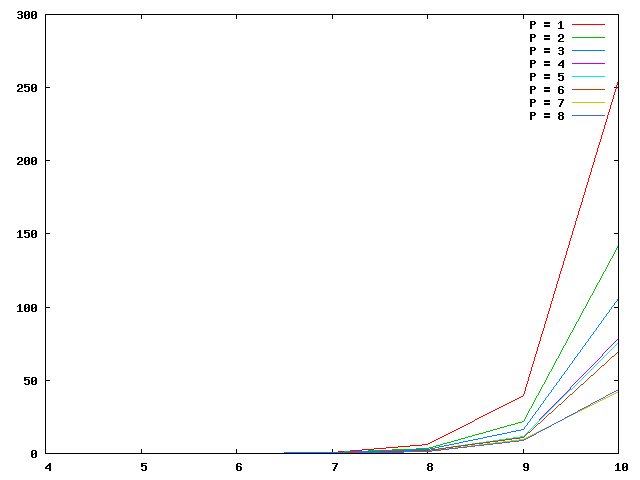
\includegraphics[width=1\textwidth]{times.png}
	\caption{Vremena izvođenja}
\end{figure}

Iz dobivenih rezultata, za dubinu koja zadovoljava uvjet da je najmanje mjereno trajanje za 8 procesora reda veličine nekoliko sekundi, uzeta je dubina $9$.

Učinkovitost paralelnog algoritma je računana prema sljedećem izrazu:

$$E = \frac{T_1}{P \cdot T_P}$$

Ubrzanje paralelnog algoritma je računato prema sljedećem izrazu:

$$S = P \cdot E$$

\begin{table}[h]
\begin{center}
\begin{tabular}{l*{4}{c}}
Broj procesora & $T_1$ & $T_P$ & Učinkovitost (E) & Ubrzanje (S)  \\
\hline
1 & 39.7422 & 39.7422 & 1.000 & 1.000 \\

2 & 39.7422 & 22.1848 & 0.896 & 1.792 \\

3 & 39.7422 & 16.6265 & 0.797 & 2.391 \\

4 & 39.7422 & 11.7097 & 0.848 & 3.392 \\

5 & 39.7422 & 11.7283 & 0.678 & 3.390 \\

6 & 39.7422 & 11.0918 & 0.597 & 3.582 \\

7 & 39.7422 & 6.6578 & 0.587 & 4.109  \\

8 & 39.7422 & 6.8622 & 0.560 & 4.480  \\

\end{tabular}
\end{center}
\caption{Ubrzanje i učinkovitost za dubinu $9$}
\end{table}

\begin{figure}[!htb]	
	\centering
	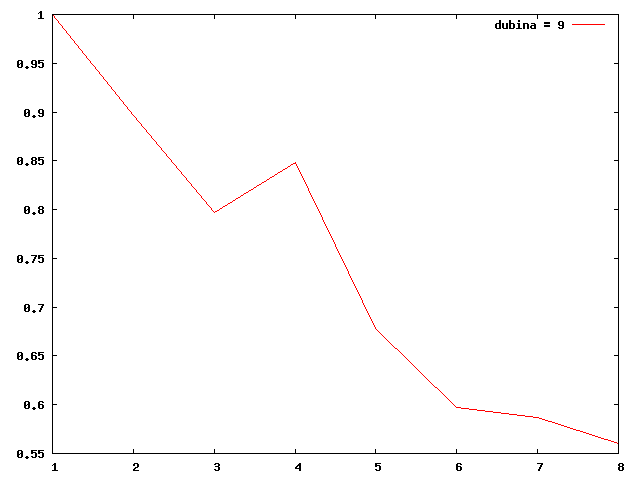
\includegraphics[width=1\textwidth]{E.png}
	\caption{Učinkovitost paralelnog algoritma}
\end{figure}

\clearpage

\begin{figure}[!htb]	
	\centering
	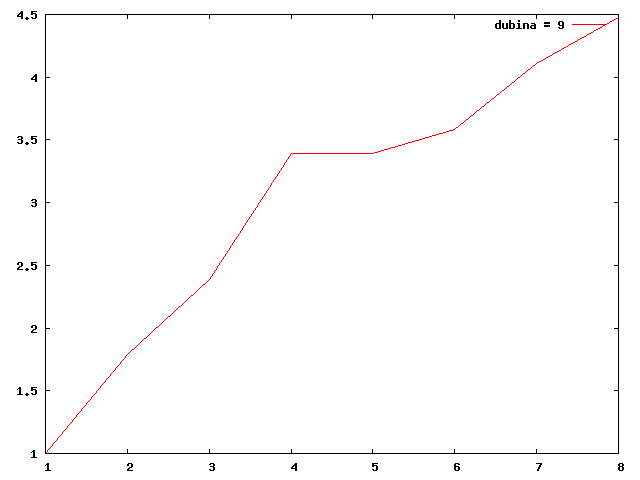
\includegraphics[width=1\textwidth]{S.png}
	\caption{Ubrzanje paralelnog algoritma}
\end{figure}

\section{Zaključak}

Za dubinu $9$, na grafovima možemo primijetiti neočekivano ponašanje prilikom korištenja $4$ procesora. Te anomalije možemo pripisati kašnjenju prilikom komunikacije. Naime, može se dogoditi da se paralelni algoritam izvodi dulje od sljednog algoritma ili paralelnog algoritma s malenim brojem dostupnih procesora zbog vremena kojeg utroši na slanje/primanje podataka.

Kao konačni zaključak se može kazati, da iz priloženih podataka, vidimo da je paralelni algoritam skalabilan budući da povećanjem broja procesora, nakon konačnog broja procesora, ubrzanje monotono raste.

\end{document}
